% https://tex.stackexchange.com/a/153934/173708
\documentclass[article, a4paper, 12pt, oneside]{memoir}
\usepackage{tikz}
\usetikzlibrary{mindmap}
\pagestyle{empty}
\begin{document}
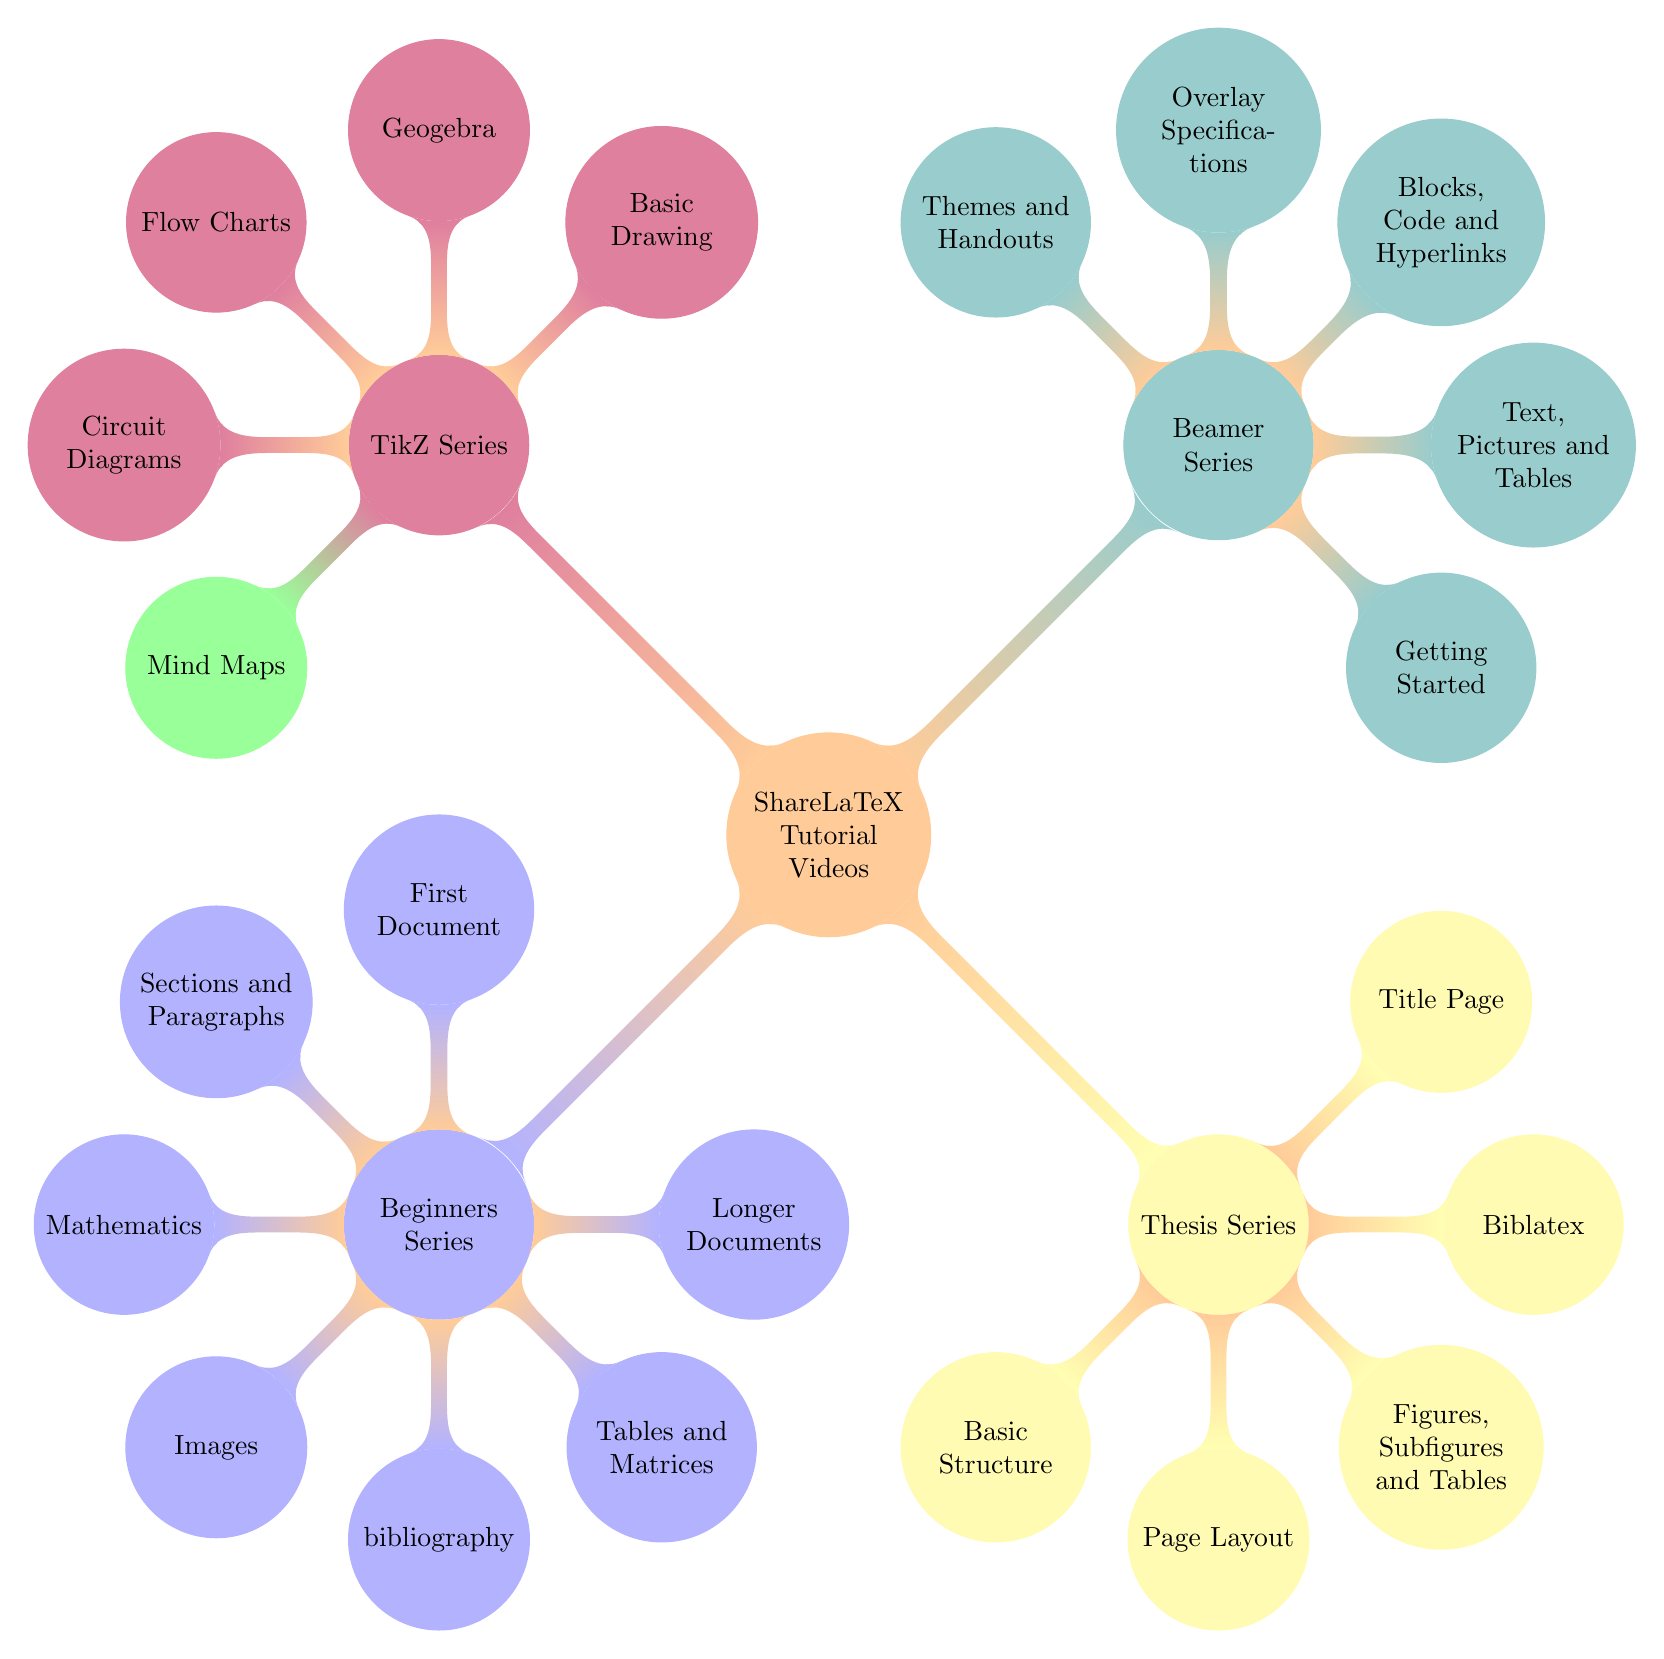
\begin{tikzpicture}[grow cyclic, text width=2cm, align=flush center, every node/.style=concept, concept color=orange!40,
level 1/.style={level distance=7cm,sibling angle=90},
level 2/.style={level distance=4cm,sibling angle=45}]

\node{ShareLaTeX Tutorial Videos}
   child [concept color=blue!30] { node {Beginners Series}
        child { node {First Document}}
        child { node {Sections and Paragraphs}}
        child { node {Mathematics}}
        child { node {Images}}
        child { node {bibliography}}
        child { node {Tables and Matrices}}
        child { node {Longer Documents}}
    }
    child [concept color=yellow!30] { node {Thesis Series}
        child { node {Basic Structure}}
        child { node {Page Layout}}
        child { node {Figures, Subfigures and Tables}}
        child { node {Biblatex}}
        child { node {Title Page}}
    }
    child [concept color=teal!40]  { node {Beamer Series}
        child { node {Getting Started}}
        child { node {Text, Pictures and Tables}}
        child { node {Blocks, Code and Hyperlinks}}
        child { node {Overlay Specifications}}
        child { node {Themes and Handouts}}
    }
    child [concept color=purple!50] { node {TikZ Series}
        child { node {Basic Drawing}}
        child { node {Geogebra}}
        child { node {Flow Charts}}
        child { node {Circuit Diagrams}}
        child [concept color=green!40]  { node {Mind Maps}}
    };

\end{tikzpicture}

\end{document}